Rysunki ~\ref{fig:rys1} - ~\ref{fig:rys5} przedstawiają wykresy dla lasera VCSEL 850\,nm. \\
\begin{table}
\begin{center}
\caption{ Wyznaczone wartośc prądu progowego $I_{\mathrm{th}}$ w różnych temperaturach $T$ dla lasera VCSEL 850\,nm. }
\begin{tabular}{ | C{1.5cm}|  C{3.0cm} | C{1.5cm} | C{3.0cm}| C{1.5cm} | C{3.0cm}|}
\hline
$T$ [K] &   $I_{\mathrm{th}}$ [mA]  &  $T$ [K] &   $I_{\mathrm{th}}$ [mA]  &  $T$ [K] &   $I_{\mathrm{th}}$ [mA] 	\\ \hline
283      &   1.70 $\pm$ 0.03  & 288      &   1.67 $\pm$ 0.03   & 293		 &   1.60 $\pm$ 0.03  \\ \hline
298		 &   1.55 $\pm$ 0.04  & 303		 &   1.59 $\pm$ 0.03  & 308		 &   1.63 $\pm$ 0.03  \\ \hline
313		 &   1.65 $\pm$ 0.03  & 318		 &   1.68 $\pm$ 0.04  & 323		 &   1.73 $\pm$ 0.04  \\ \hline
328		 &   1.83 $\pm$ 0.04  & 333		 &   1.89 $\pm$ 0.04  & 338		 &   2.01 $\pm$ 0.04  \\ \hline
343		 &   2.14 $\pm$ 0.04  & 348		 &   2.24 $\pm$ 0.05  & 353		 &   2.38 $\pm$ 0.05  \\ \hline
358		 &   2.57 $\pm$ 0.05  & 363		 &   2.74 $\pm$ 0.07  \\ \cline{1-4}
\end{tabular}
\end{center}
\end{table}
\begin{figure}
\center
  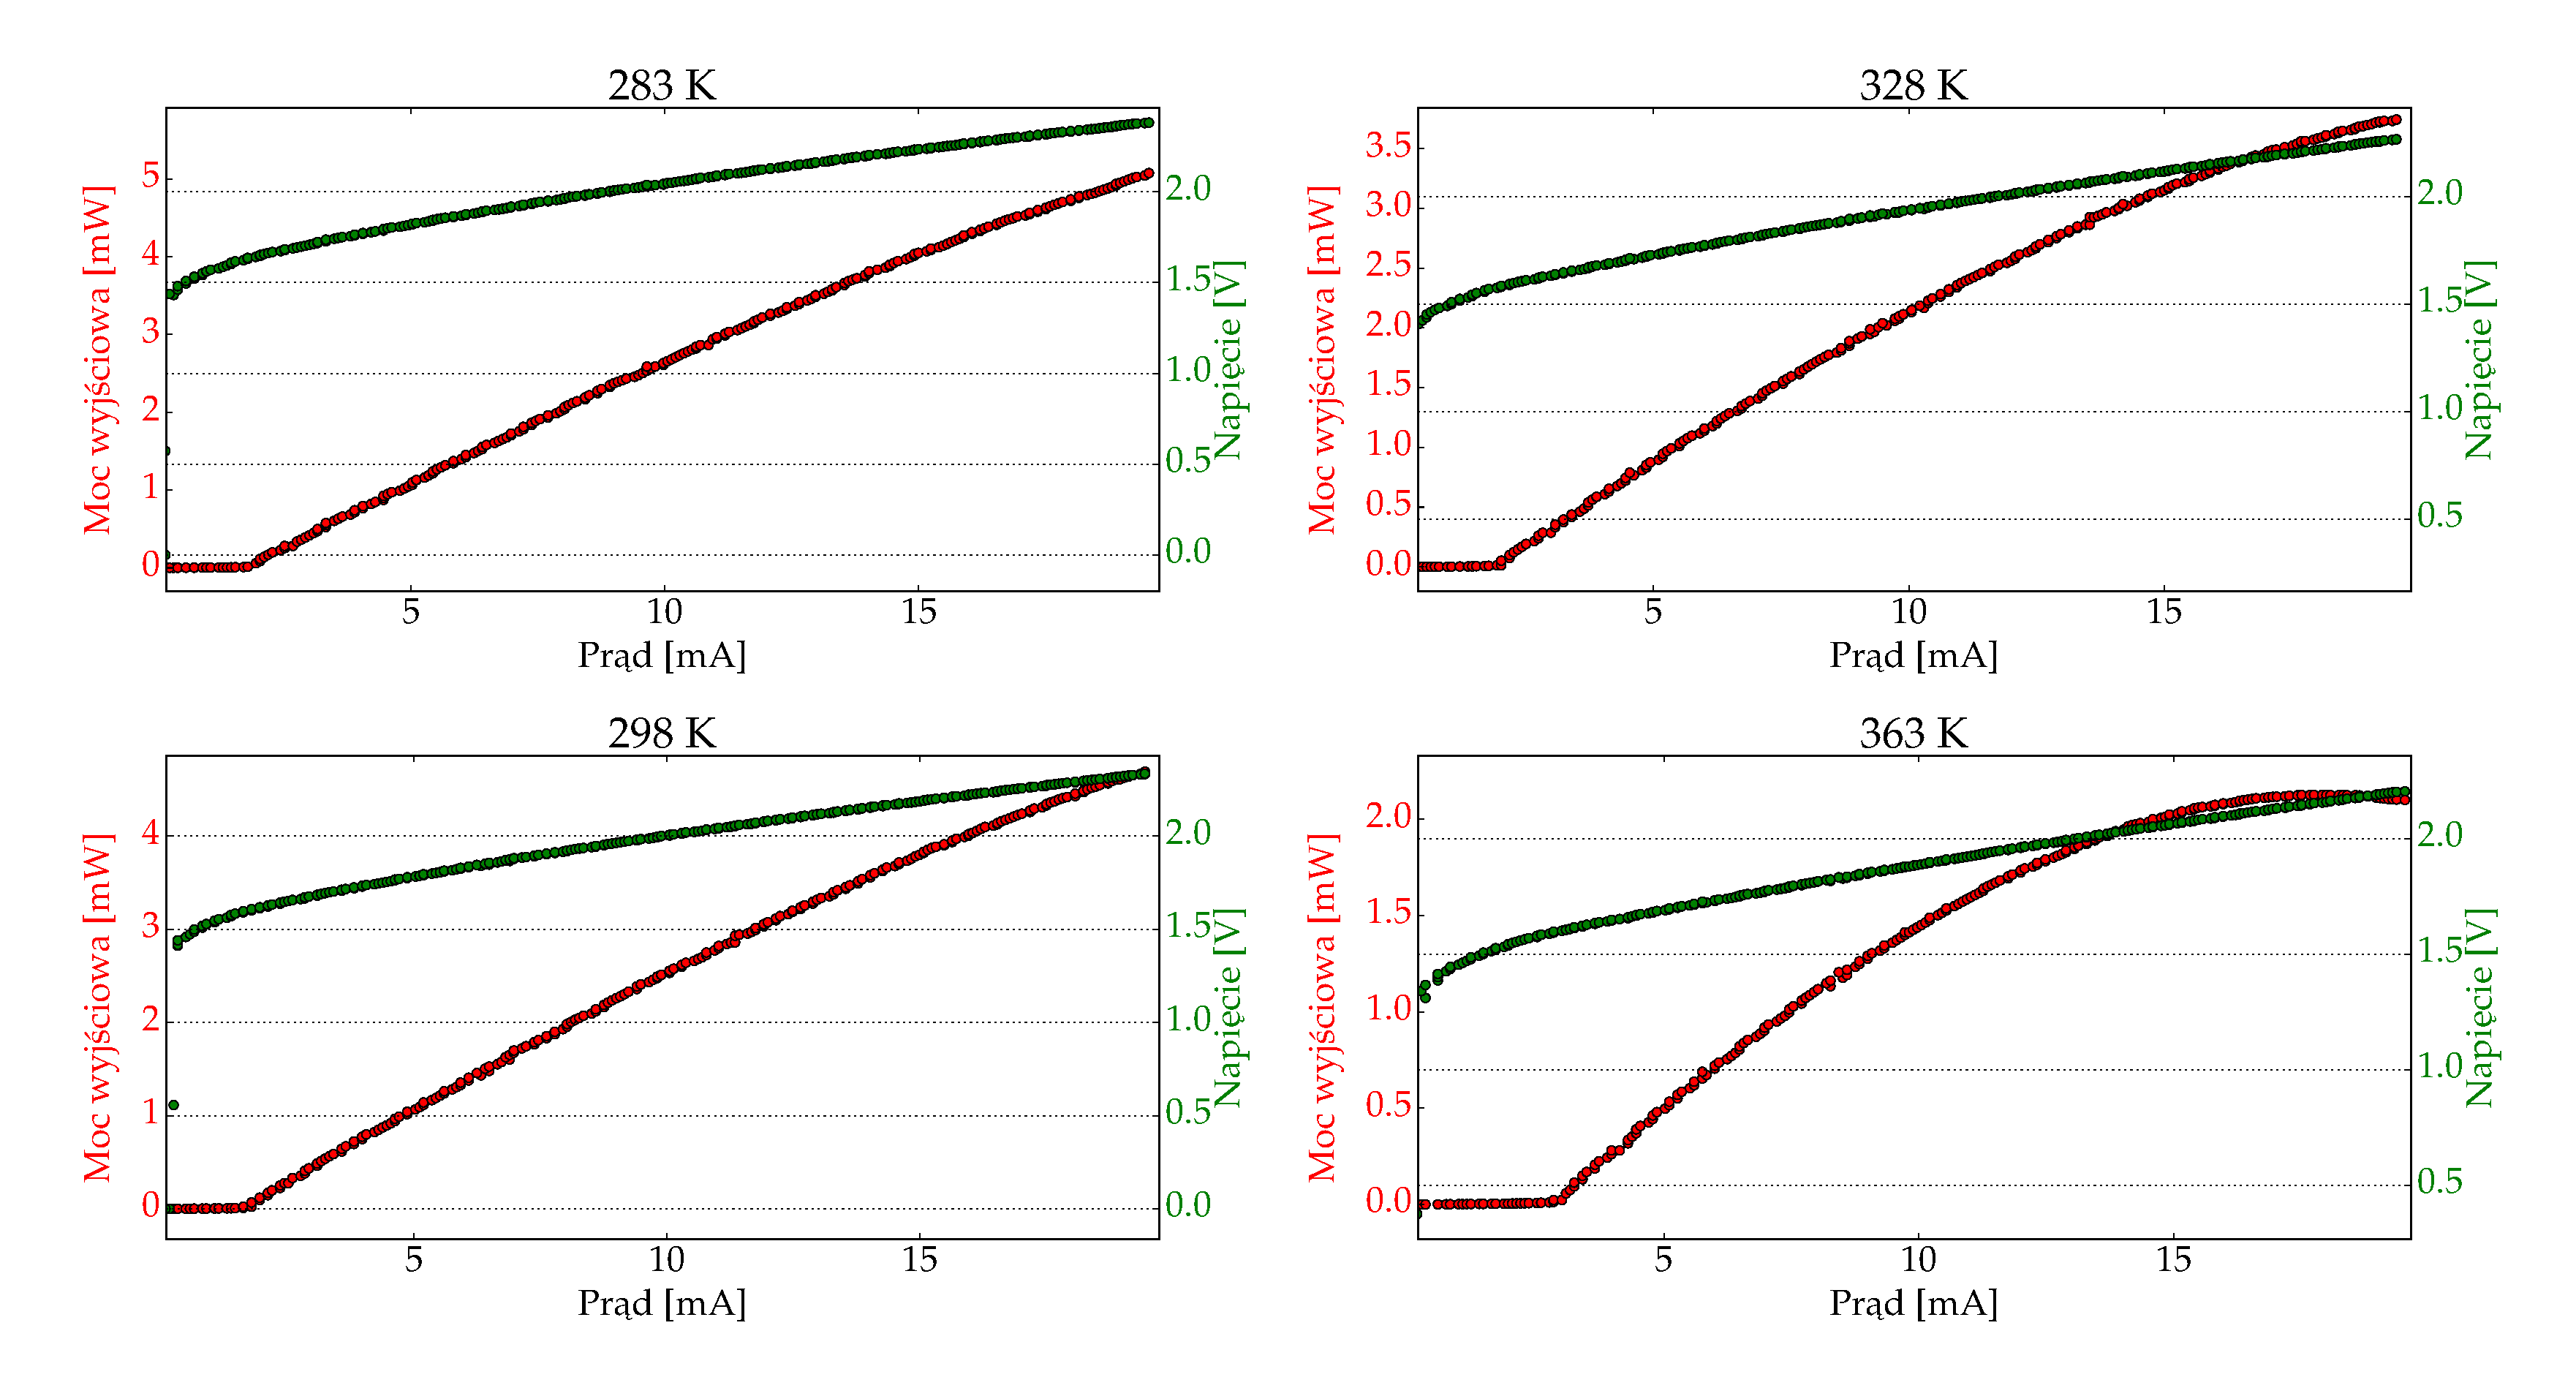
\includegraphics[scale=0.30]{plot_vcsel_850/plot_ivl_4.eps}
  \caption{Sprawność VCSEL 850.} 
  \label{fig:rys1}
\end{figure}
\begin{figure}
\center
  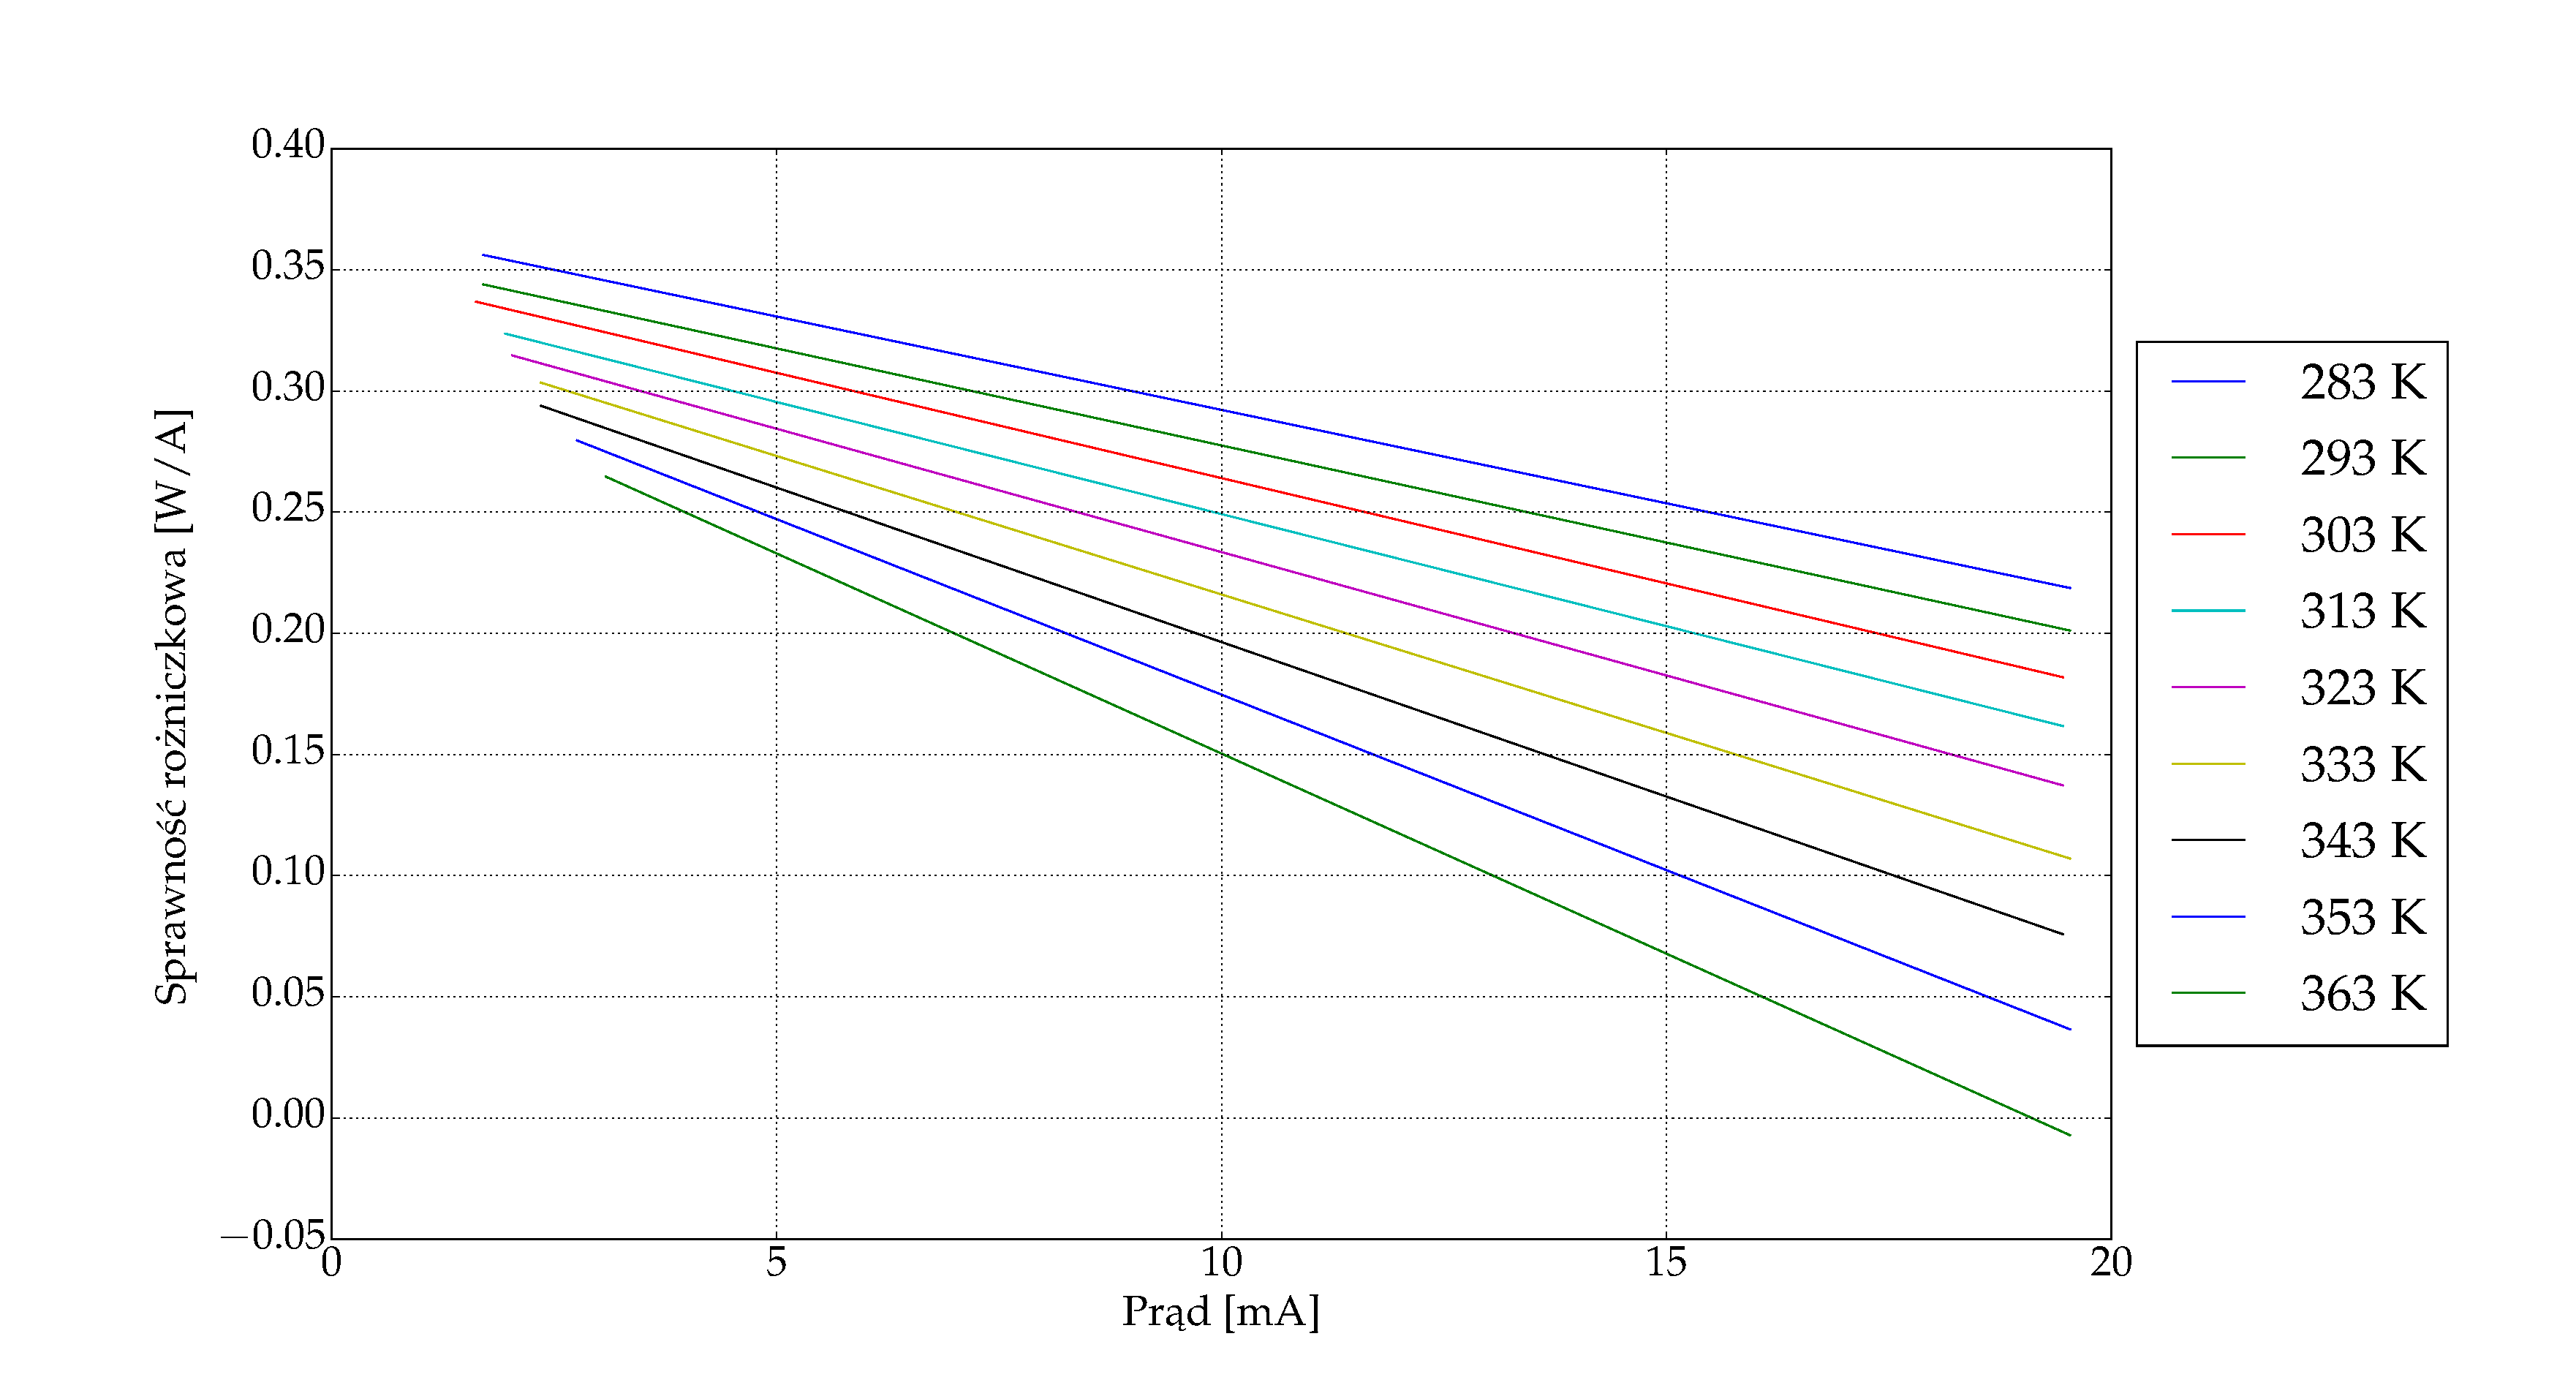
\includegraphics[scale=0.30]{plot_vcsel_850/plot_eff_all_via_current.eps}
  \caption{Sprawność VCSEL 850 w funkcji prądu.}
  \label{fig:rys2}
\end{figure}
\begin{figure}
\center
  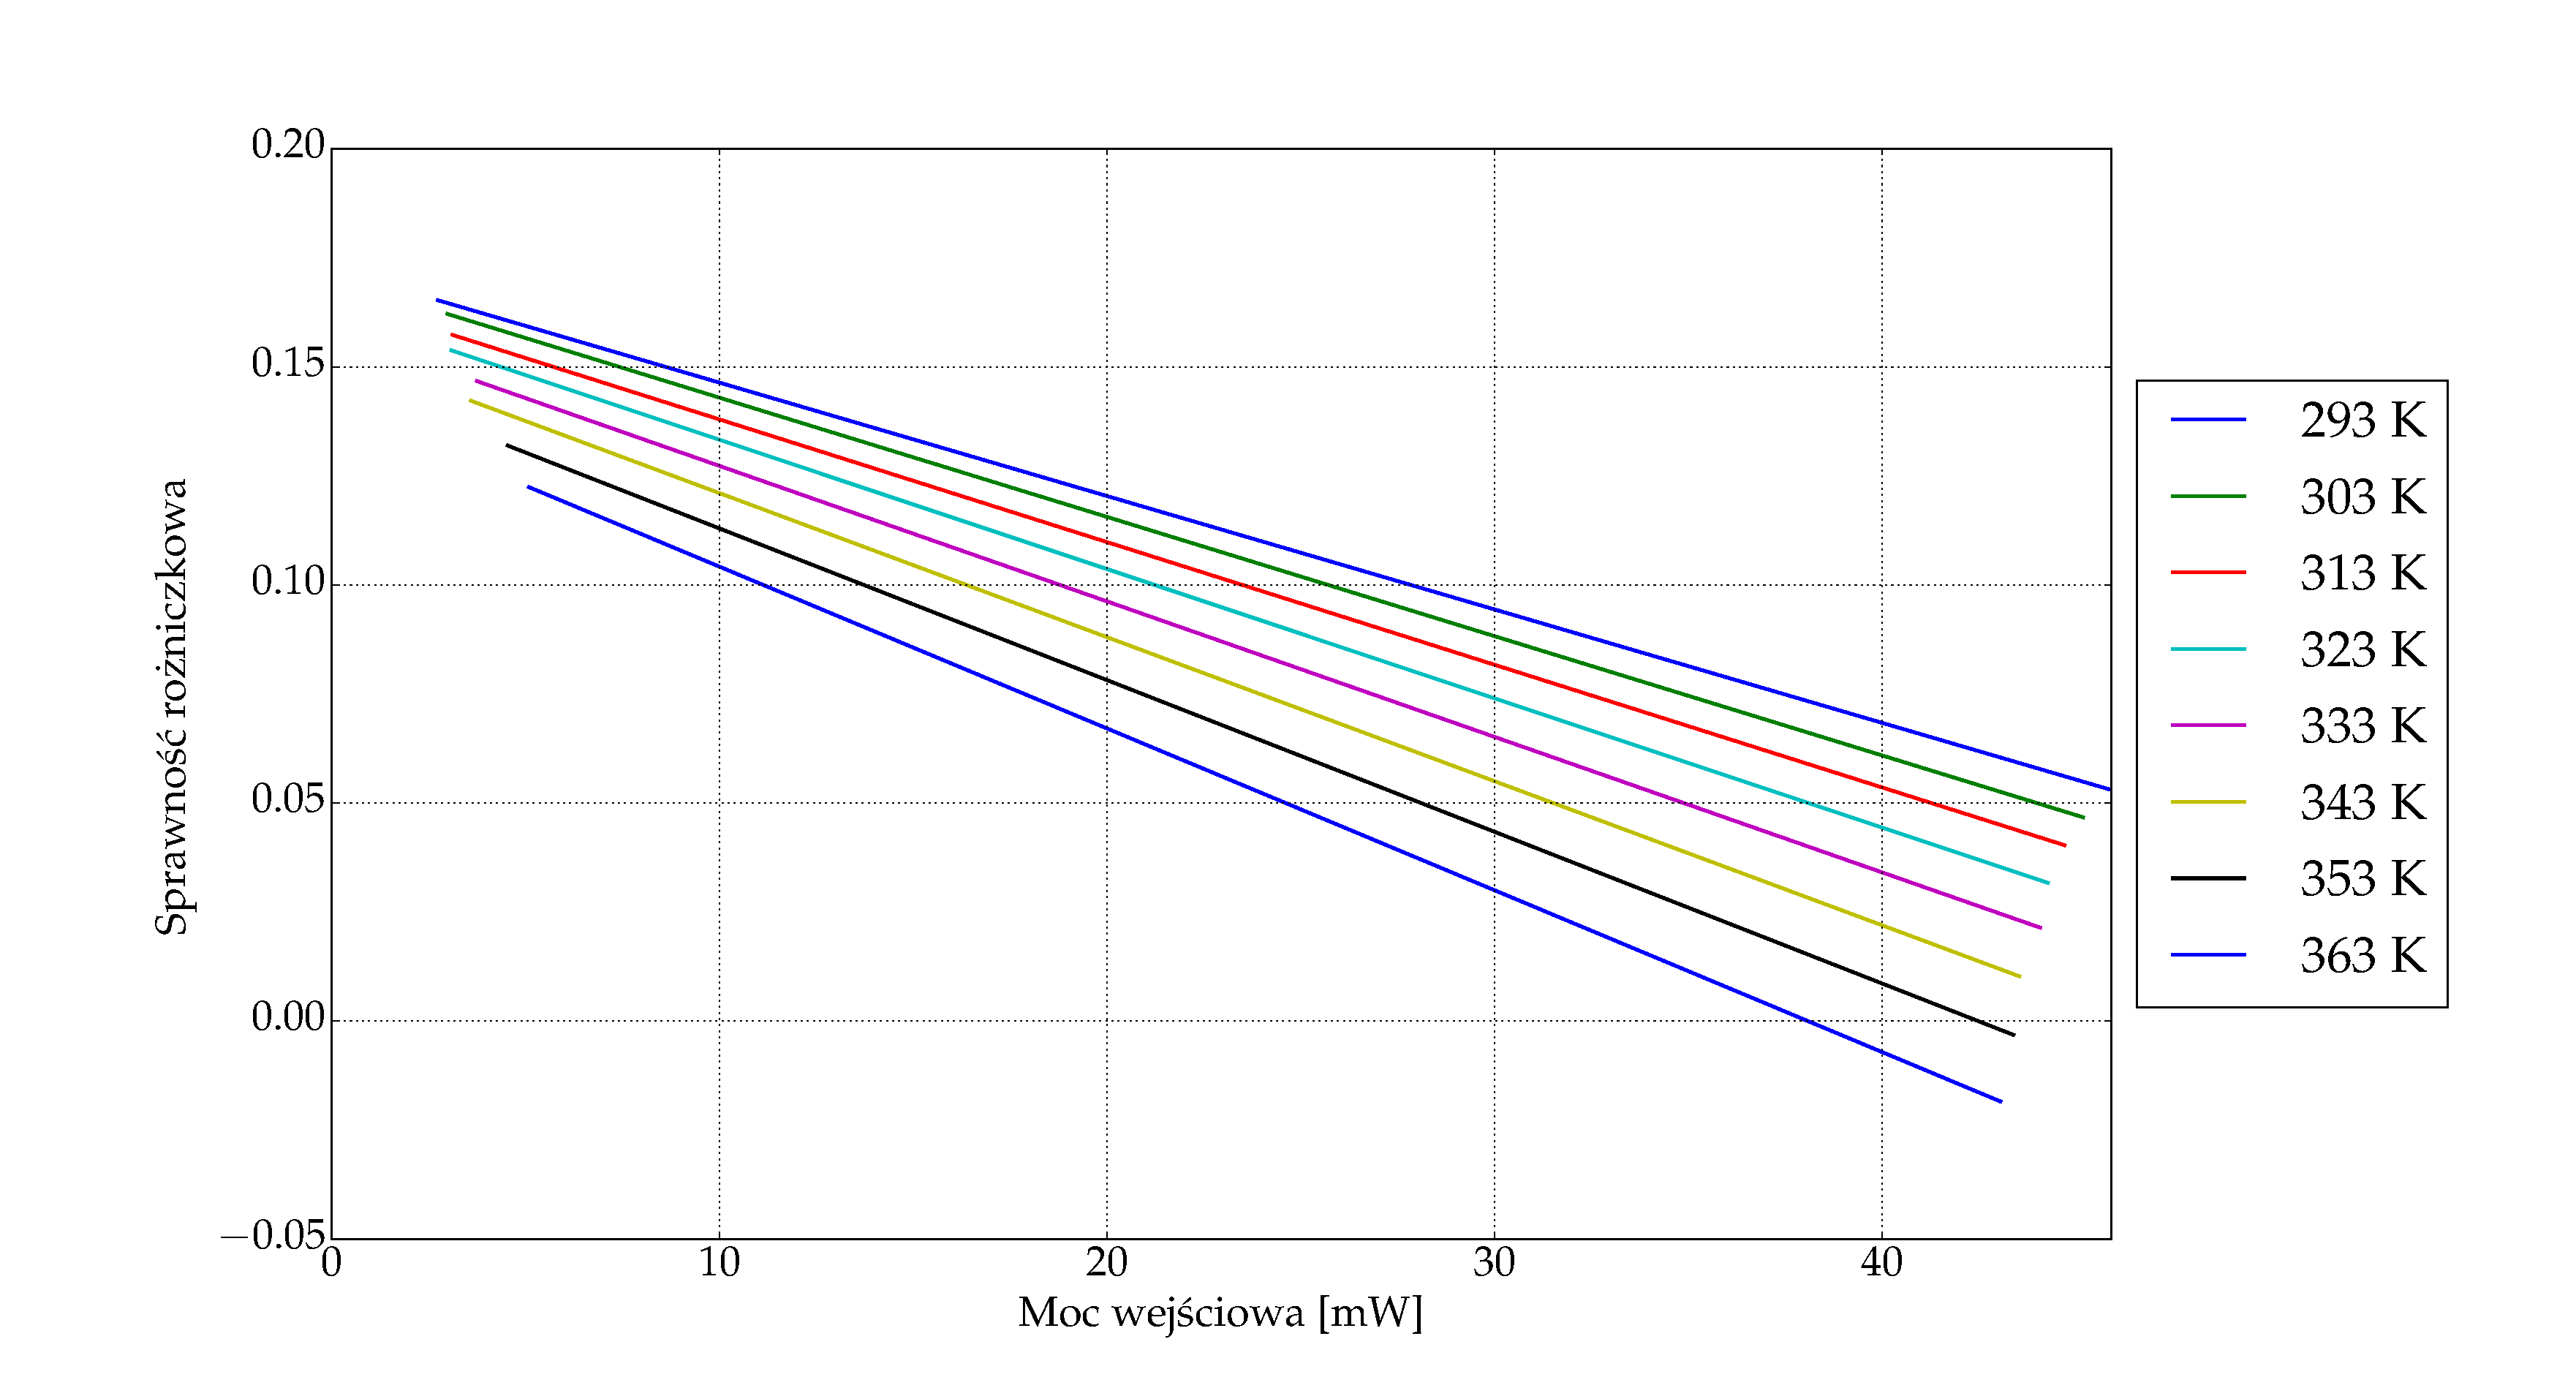
\includegraphics[scale=0.30]{plot_vcsel_850/plot_eff_all_via_power.eps}
  \label{fig:rys3}
  \caption{Sprawność VCSEL 850 w funkcji mocy wejściowej.}
\end{figure}
\begin{figure}
\center
  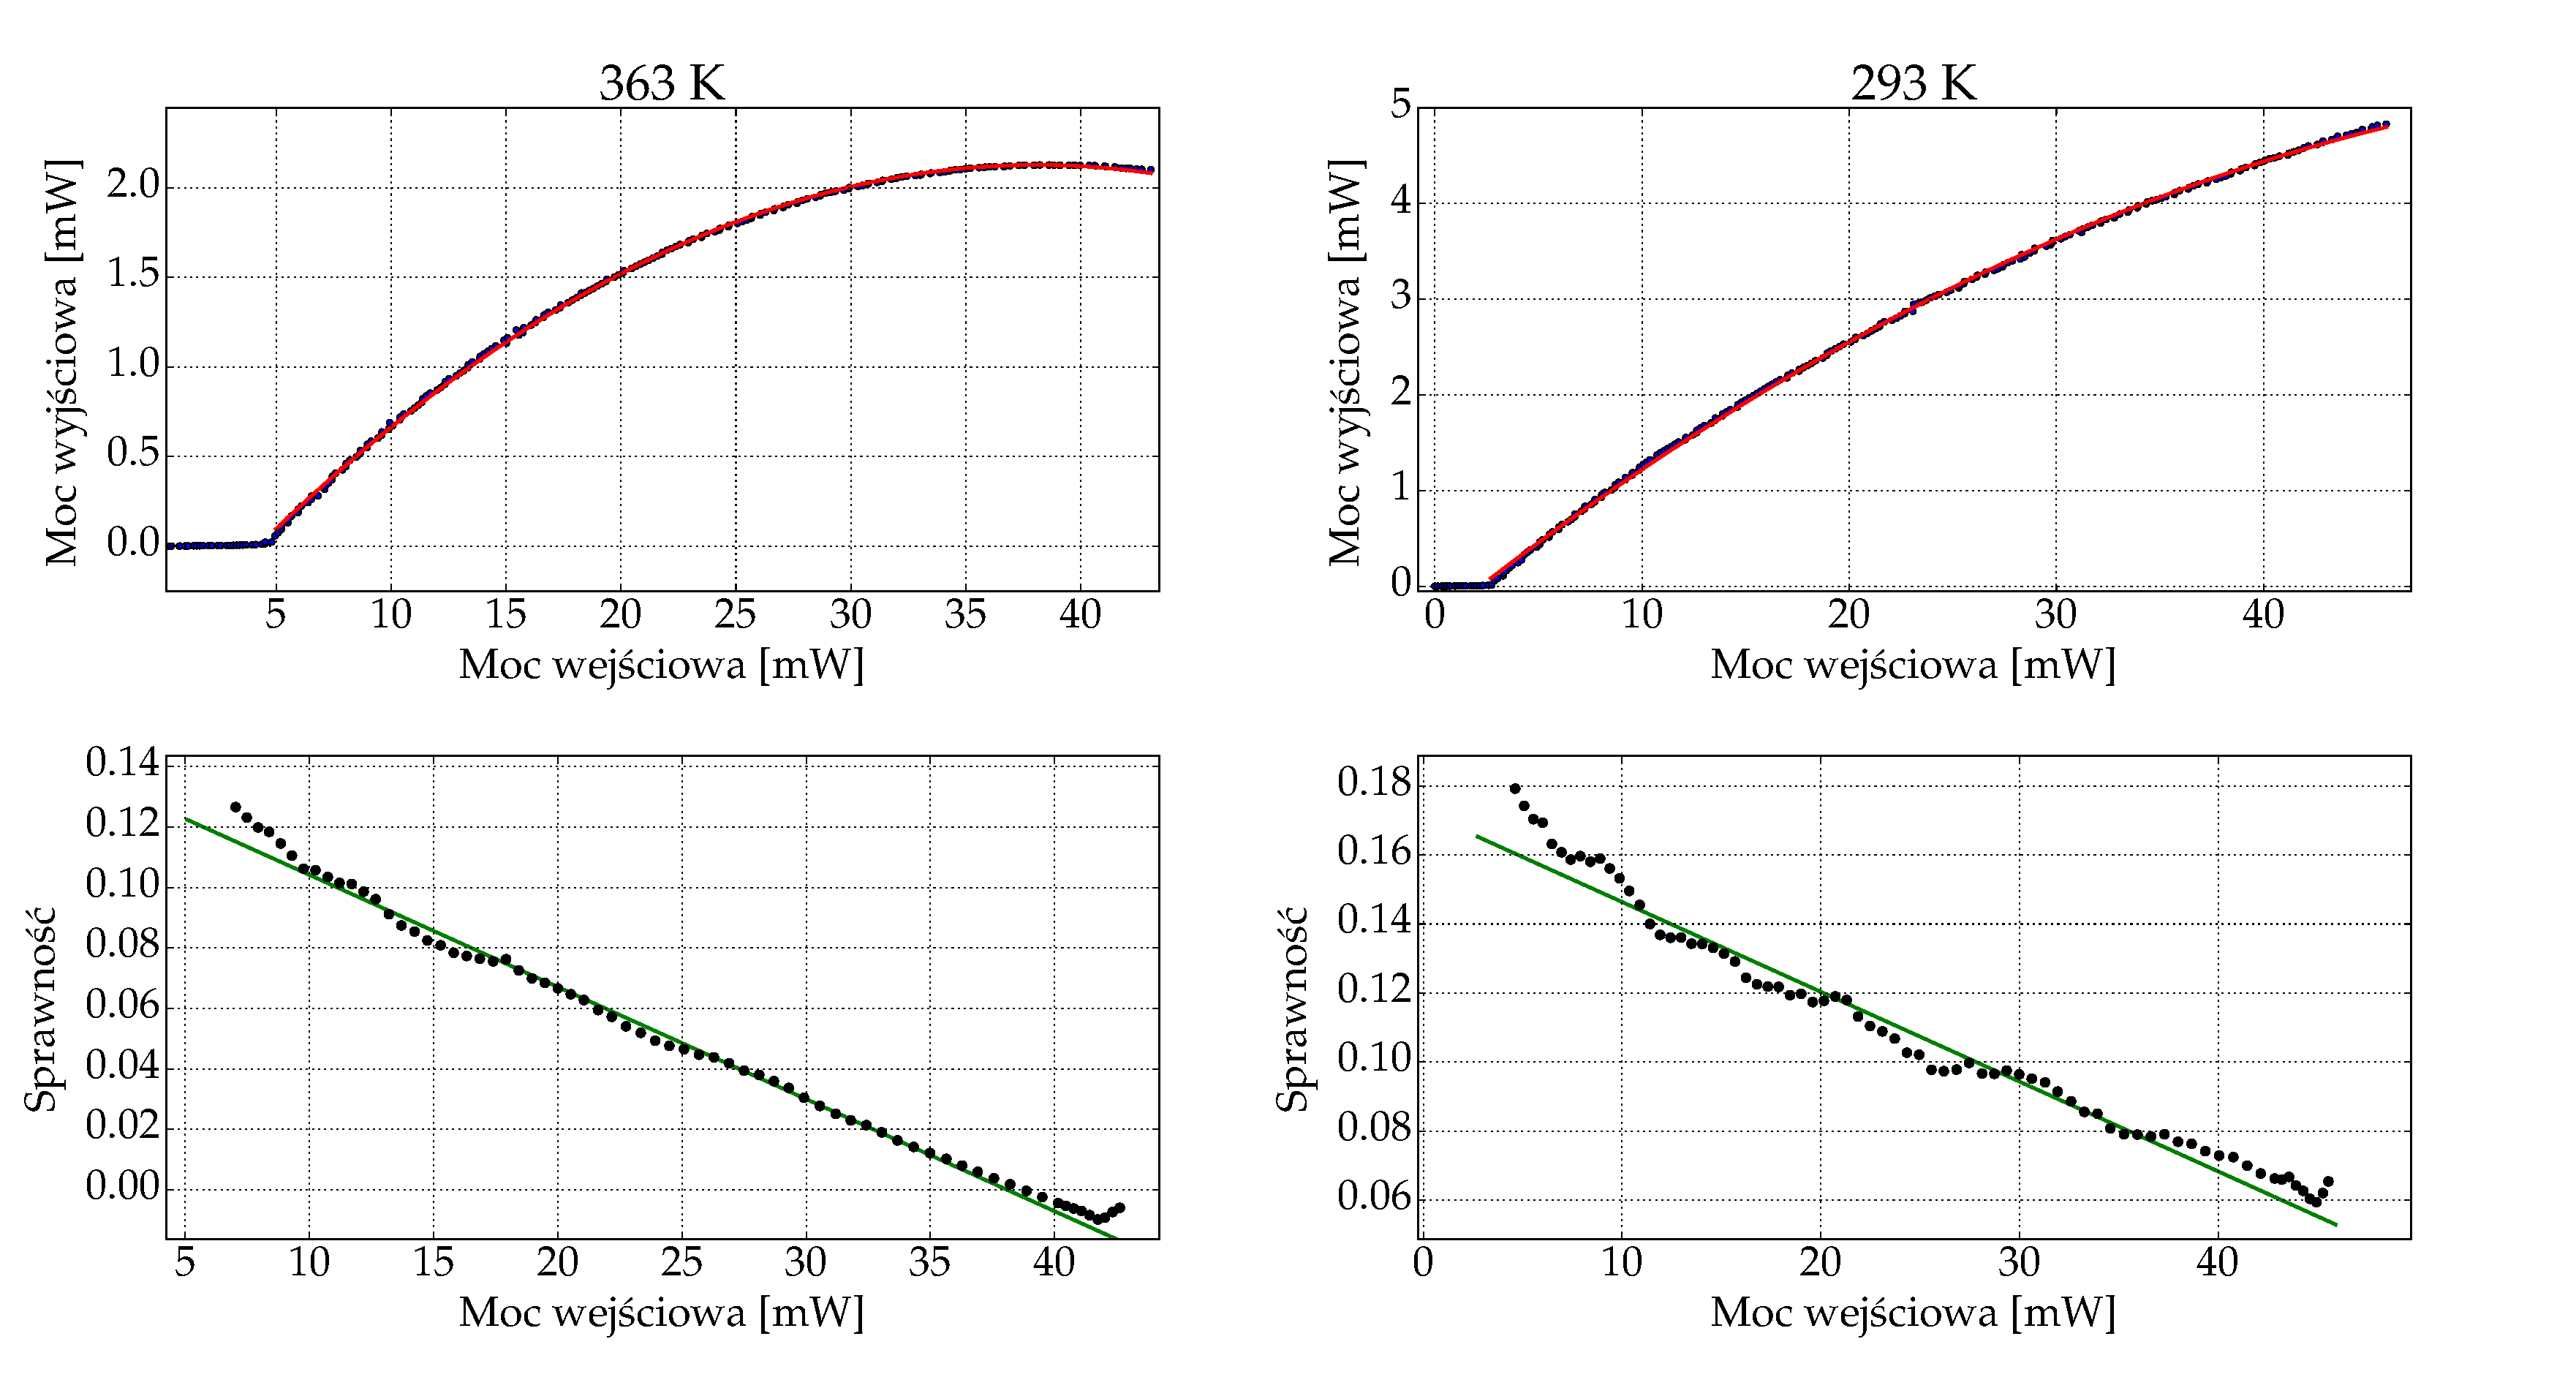
\includegraphics[scale=0.30]{plot_vcsel_850/plot_eff_20_90_via_power.eps}
  \label{fig:rys4}
  \caption{Sprawność VCSEL 850 dla temperatury 293\,K i 363\,K.} 
\end{figure}
\begin{figure}
\center
  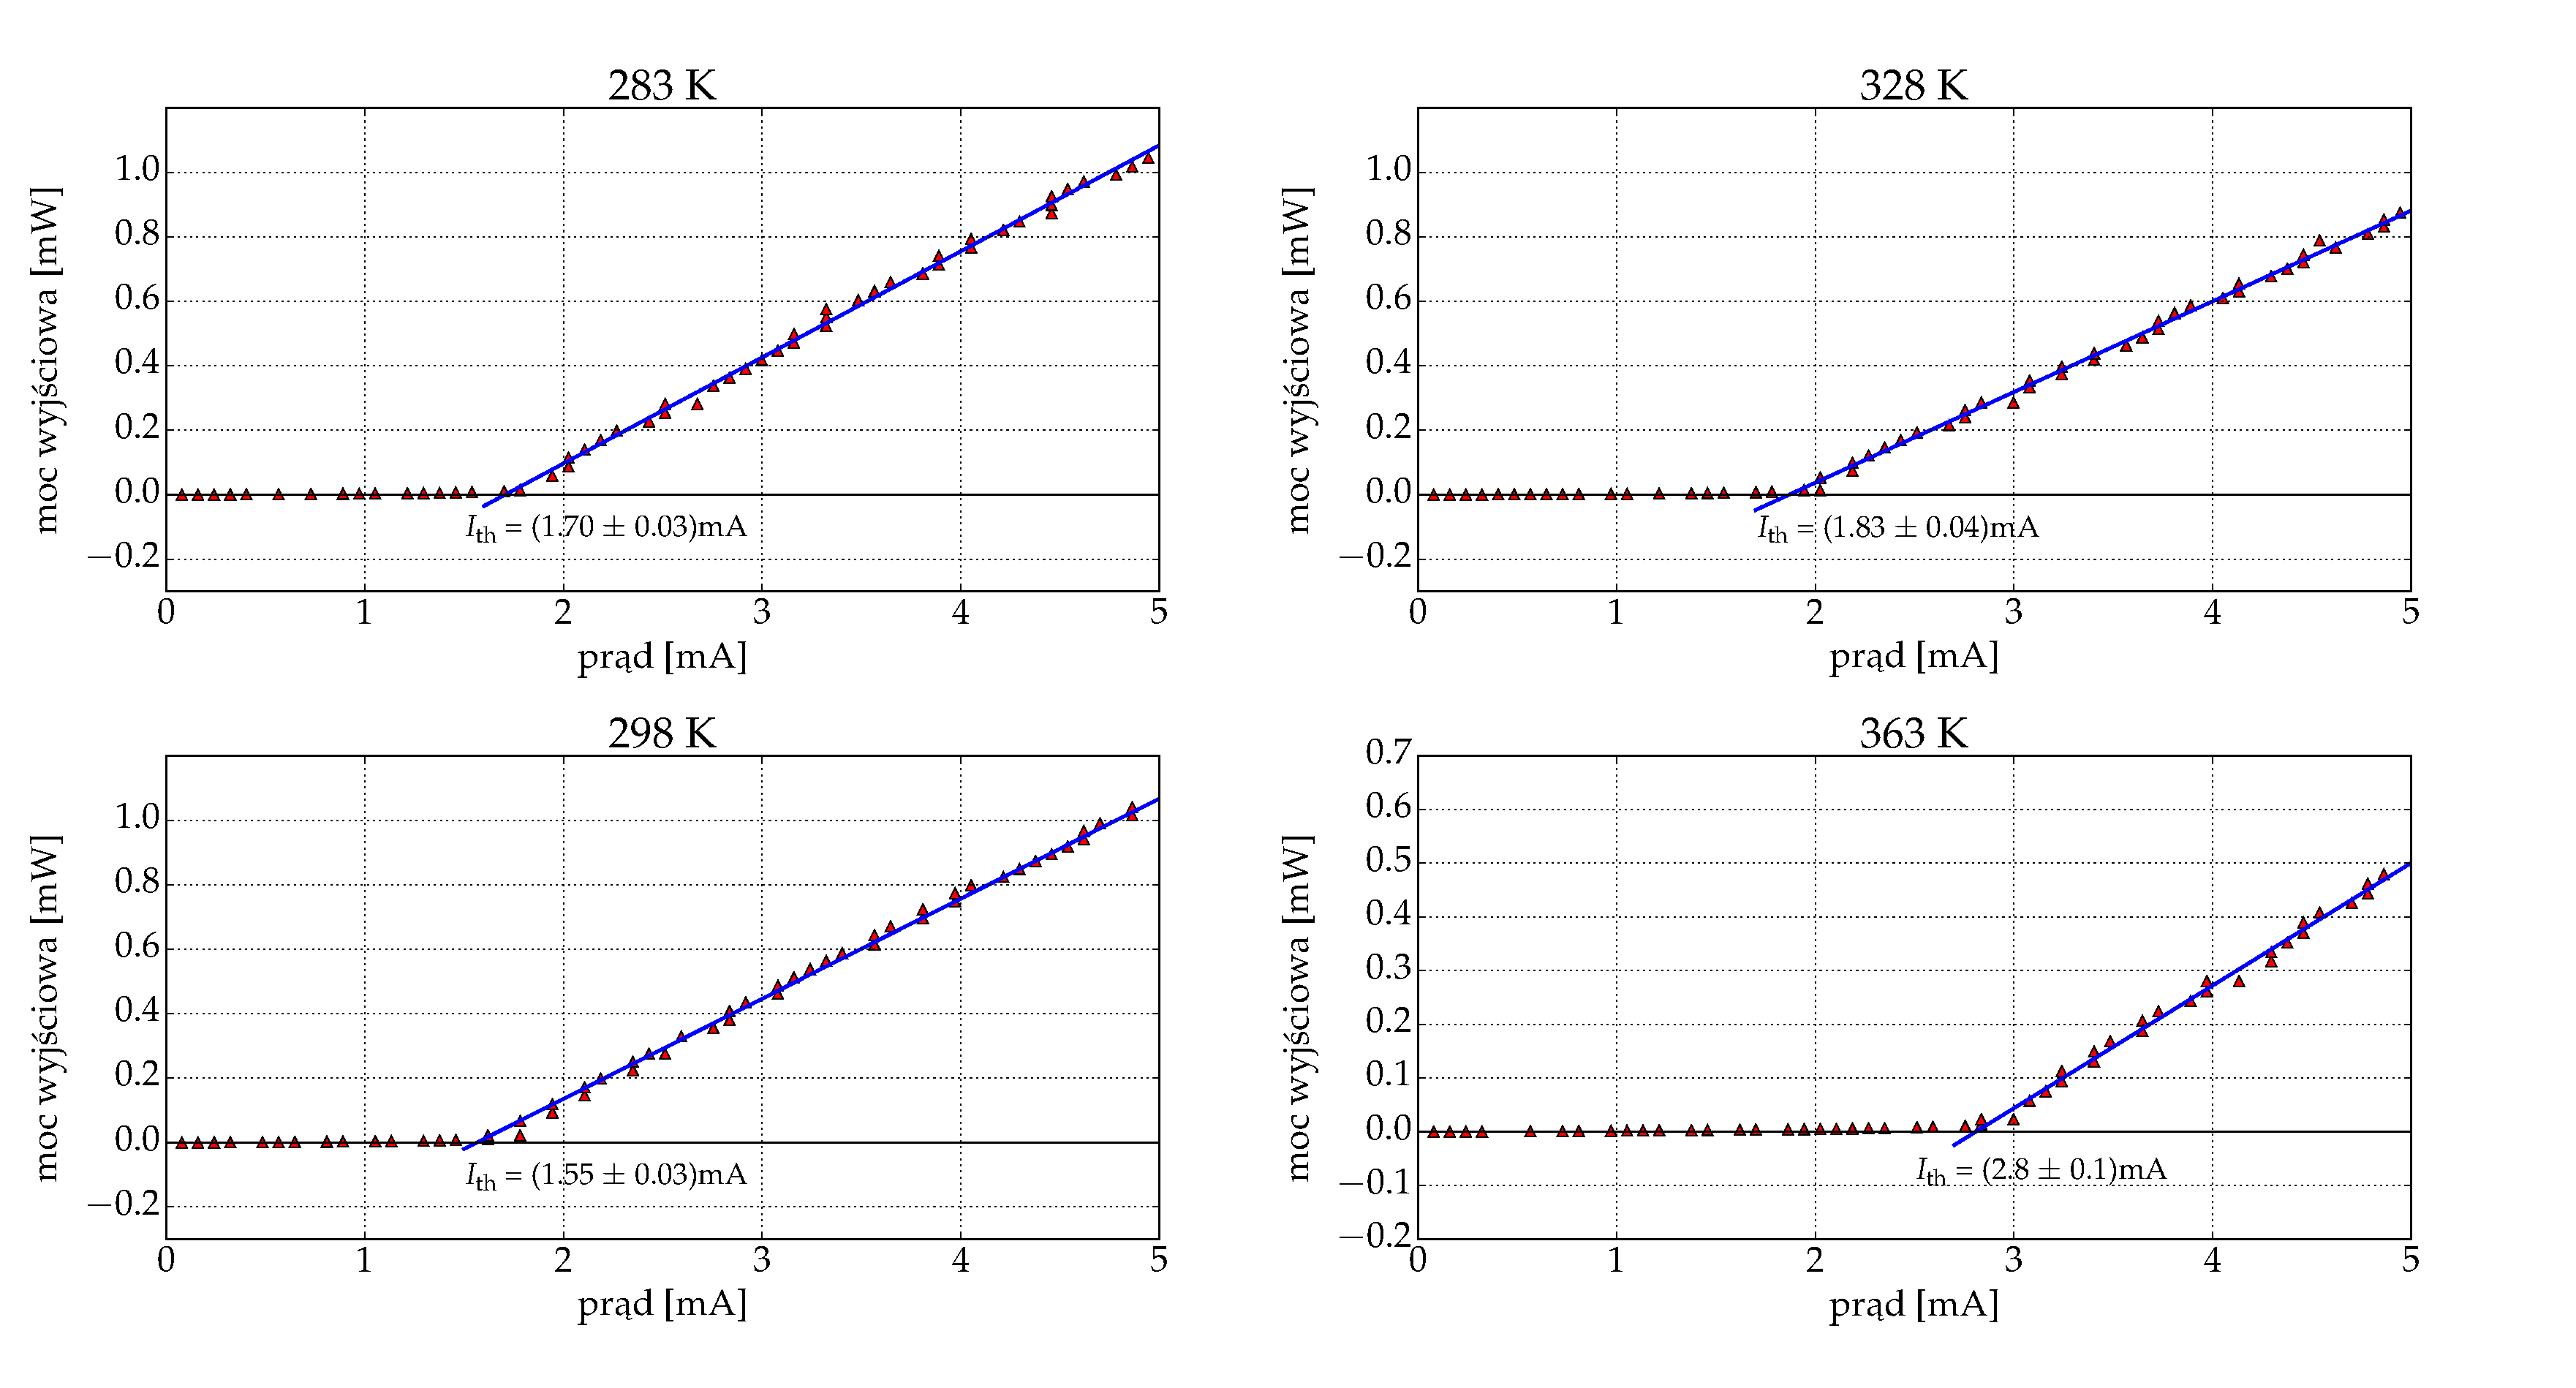
\includegraphics[scale=0.30]{plot_vcsel_850/plot_fit_i_th.eps}
  \caption{Wykres prądu progowego od temperatury z wyznaczonymi progami prądu.}
  \label{fig:rys5}
\end{figure}
\begin{figure}
\center
  % This file was created by matplotlib2tikz v0.6.0.
\begin{tikzpicture}

\begin{axis}[
xlabel={Temperatura [K]},
ylabel={Prąd progowy [mA]},
xmin=280, xmax=370,
ymin=1.4, ymax=3,
axis on top,
width=16cm,
height=9cm,
xmajorgrids,
ymajorgrids
]
\path [draw=red] (axis cs:283,1.67)
--(axis cs:283,1.73);

\path [draw=red] (axis cs:288,1.64)
--(axis cs:288,1.7);

\path [draw=red] (axis cs:293,1.57)
--(axis cs:293,1.63);

\path [draw=red] (axis cs:298,1.51)
--(axis cs:298,1.59);

\path [draw=red] (axis cs:303,1.56)
--(axis cs:303,1.62);

\path [draw=red] (axis cs:308,1.6)
--(axis cs:308,1.66);

\path [draw=red] (axis cs:313,1.62)
--(axis cs:313,1.68);

\path [draw=red] (axis cs:318,1.64)
--(axis cs:318,1.72);

\path [draw=red] (axis cs:323,1.69)
--(axis cs:323,1.77);

\path [draw=red] (axis cs:328,1.79)
--(axis cs:328,1.87);

\path [draw=red] (axis cs:333,1.85)
--(axis cs:333,1.93);

\path [draw=red] (axis cs:338,1.96)
--(axis cs:338,2.04);

\path [draw=red] (axis cs:343,2.1)
--(axis cs:343,2.18);

\path [draw=red] (axis cs:348,2.19)
--(axis cs:348,2.29);

\path [draw=red] (axis cs:353,2.33)
--(axis cs:353,2.43);

\path [draw=red] (axis cs:358,2.52)
--(axis cs:358,2.62);

\path [draw=red] (axis cs:363,2.67)
--(axis cs:363,2.81);

\addplot [red, mark=-, mark size=3, mark options={solid}, only marks]
table {%
283 1.67
288 1.64
293 1.57
298 1.51
303 1.56
308 1.6
313 1.62
318 1.64
323 1.69
328 1.79
333 1.85
338 1.96
343 2.1
348 2.19
353 2.33
358 2.52
363 2.67
};
\addplot [red, mark=-, mark size=3, mark options={solid}, only marks]
table {%
283 1.73
288 1.7
293 1.63
298 1.59
303 1.62
308 1.66
313 1.68
318 1.72
323 1.77
328 1.87
333 1.93
338 2.04
343 2.18
348 2.29
353 2.43
358 2.62
363 2.81
};
\addplot [red, mark=*, mark size=3, mark options={solid,draw=black}, only marks]
table {%
283 1.7
288 1.67
293 1.6
298 1.55
303 1.59
308 1.63
313 1.65
318 1.68
323 1.73
328 1.83
333 1.89
338 2
343 2.14
348 2.24
353 2.38
358 2.57
363 2.74
};
\end{axis}

\end{tikzpicture}
  \caption{Wykres prądu progowego od temperatury.}
  \label{fig:rys6}
\end{figure}
